\documentclass[../document.tex]{subfiles}

\begin{document}

\section{Project Plan}
\subsection{Introduction}
In this chapter we will present our organisational plan, including the methodology that we use and how we plan to split the project in manageable phases. The list of risks accompanied by their mitigation plan, as well as quality assurance is included in the latter part of this chapter.

This chapter will help our team compare the initial plan of the project with the actual work that we have done after the twelve weeks have passed, allowing for good self-evaluation. Furthermore, we believe that a plan is necessary to maintain good pacing and finish the project on time.

\subsection{Resources}
Here we will list the resources available for the team during the course of this project.

\subsubsection{Human Resources}
The team consists of 7 members. Assisting us will be a teaching assistant, commonly referred to as the supervisor or adviser. Finally, the customer is also involved in the project and will be assisting us during the duration of the project with feedback and advice.

\subsubsection{Time Resources}
The project spans over twelve weeks. The weekly effort calculated per team member is roughly 24.5 hours, which is rounded up to 25 hours per member per week. We split the twelve weeks into 13 time periods where we estimate to spend 50 hours in the first period and 175 hours in all the other periods. Therefore the total amount of time that is to be spent on the project, as an upper estimate is: 12 time periods * 175 person hours + 50 person hours , which equals to 2150 working hours during the course of the project.
\newline \ \newline
The project will have to meet two important deadlines:
\begin{itemize}
\item
October 17th: A pre-delivery to the examiner needs to be handed in to the group supervisor and the external examiner. The pre-delivery consists of documentation that will familiarize the external examiner with our project.
\item
November 20th: Between 9:15 and 14:00 we will be holding the presentation of our project, which also includes a demonstration as well as the final hand-in to the supervisor and the present examiners. An electronic copy will also be handed in to the project coordinator a day before the final presentation.
\end{itemize}

\subsection{Project Organization}
In this section we will list our project organization. This includes a short interlude to our methodology and the key roles identified in the group.

\subsubsection{Methodology - Scrum}
The team will be organized using the Agile methodology. To be more precise, we are going to use Scrum. More details about why we chose Scrum and the normal procedures used in an agile environment can be found in \subsubfullref{the_scrum_model}

\subsubsection{Roles}
The team is going to have a list of roles defined in order to know the responsibilities assigned with the role. The team will only have a few permanent roles that were already assigned by the university but the rest of the roles will be taken by turn by every team member. 
\begin{figure}
\centering
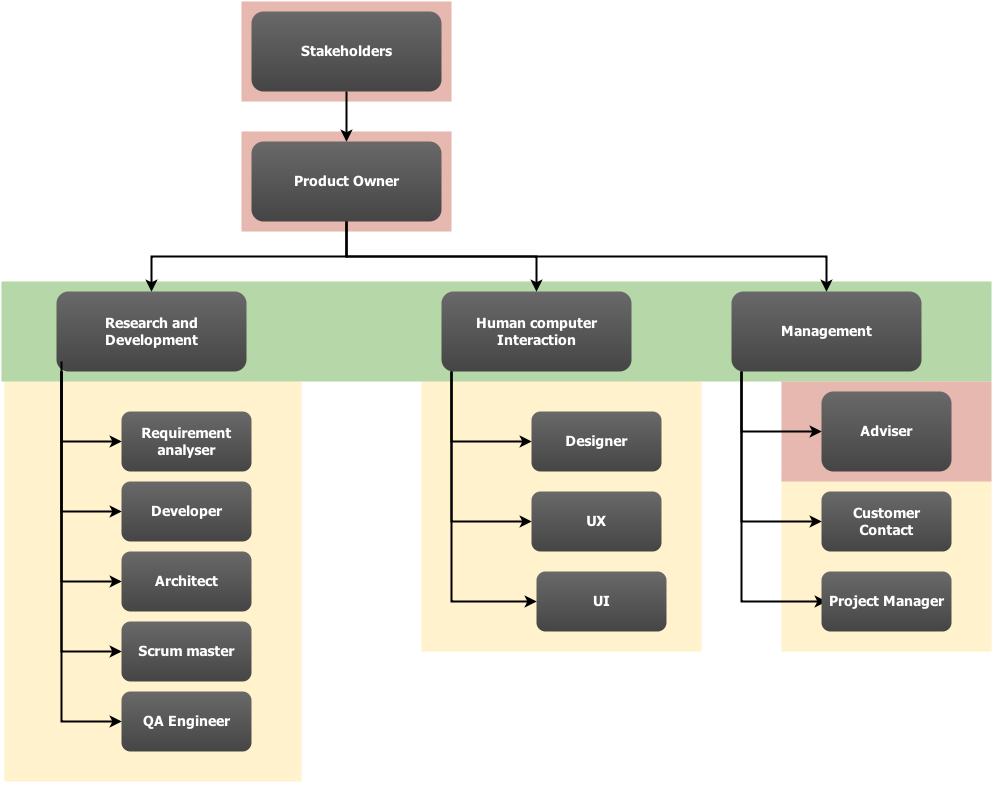
\includegraphics[width=\textwidth]{organisational-diagram.png}
\caption{Organisational Diagram}
\end{figure}

\paragraph{Adviser - Mohsen Anvaari} \ \\
The advisor serves as a one-person “steering committee” for our project. He is responsible to keep an eye on the main process of the work and to oversee that sufficient contact with the customer is maintained. The advisor must therefore regularly receive updated reports, copies of relevant work plans and technical documents from our group, so that all this can be discussed in a weekly advisor meeting. The advisor will also provide feedback, and help us with exceptional situations.


\paragraph{Product Owner - Stig Lau} \ \\
The role of the product owner is to have a vision about the product that converges all the ideas of the stakeholders in the best possible way and to maintain the collaboration between the stakeholders. The project owner is required to attend the sprint demos and provide feedback on the work done. He should also prioritise the tasks that need to be done in the following sprint. 

\paragraph{Stakeholders} \ \\
There are six stakeholders that we have identified: customer, developer, end user, advisor, course staff and hardware suppliers. Out of these the main stakeholders are the customer, the developer and the advisor. The stakeholders hold different interests in the project, however, in order for our project to be successful, communication between the main stakeholders is mandatory. The quality assurance documentation, at the end of this chapter, dictates the frequency of the meetings as well as how the meetings will be held. Furthermore, the architectural documentation describes all the stakeholders further in depth.

\paragraph{Customer Contact} \ \\
The customer contact takes care of the communication with the customer and makes sure that the product owner is informed in advance about meetings, as well as questions or issues related to the product. He respects the procedures related to how to set up a meeting with the customer. The customer contact is also responsible for collaboration with the adviser and makes sure that he gets informed about the weekly meetings. Another role of the customer contact is to reserve rooms for meetings in advance.

\paragraph{Scrum Master} \ \\
The most important role of the scrum master is to facilitate the communication and collaboration within the team. In other words the scrum master should act like a coach, making sure that team members work together as efficient as possible. Moreover, he is responsible to remove impediments to progress, facilitate meetings specific to the scrum methodology, and perform project management issues such as tracking progress. 

\paragraph{Architect} \ \\
The role of the architect is to decide, in collaboration with the remainder of the group and the customer, the architecture of the system and how the interactions between the systems should happen. The architect is also responsible in limiting the choices available during the development by choosing a standard way of pursuing application development, or by deciding on the libraries and frameworks. Another role of the architect is to foresee risks related to the procedures used in the development stage and mitigate them. 

\paragraph{Developer} \ \\
The developer is responsible for developing quality code that adheres to the project standard. The developer also needs to respect the procedures related to code commit and deploy, attend meetings and clarify specifications with the client and/or the team. Moreover, the developer also has to break down the program specification in simple logical units and translate the logic into java code. Finally, the developer needs to work as part of a team, respect and encourage teamwork, adapt the software to the new requirements and, if necessary, write documentation.

\paragraph{Requirement Analyser} \ \\
The requirement analyser is responsible for making sure that the requirements are well understood and documented. The requirements analyser must also collaborate with the product owner about the requirements and change them, should the need arise.

\paragraph{QA Engineer} \ \\
The QA engineer designs and executes testing plans, records both the current and the previous results, and compares the results. Moreover, the QA engineer is tasked with code examination and execution in different environments and reports the anomalies and issues discovered. 

\paragraph{Designer/UX/UI} \ \\
The designer designs and makes decisions related to user interfaces. He makes sure that the interface is simple and easily understood by the end-user and makes the necessary adjustments to improve the user interface should it not be satisfactory.

\subsubsection{Skills Matrix} \ \\
In order to make it easier to choose our roles during the project, we have created a skills matrix which contains most of the skills that are going to be needed during the project. Note that the skills matrix lists not only the skills each team member has, but also their confidence level in these skills. Should a team member not be confident in a particular skill they will not check it as a skill they possess.

\begin{table}[H]
\caption{Skills Matrix}
\begin{tabularx}{\textwidth}{|L{2.2cm}|X|X|L{.7cm}|X|X|X|X|}
\hline
Skills Matrix
&Audun
&Catalin
&Julie
&Maria
&Nenad
&Niklas
&Shimin
\\ \hline Planning
&x
&x
&x
&x
&x
&x
&x
\\ \hline Documentation
&x
&x
&x
&x
&x
&x
&x
\\ \hline Requirement Specification
&x
&
&
&
&x
&x
&x
\\ \hline Java
&x
&x
&x
&x
&x
&x
&x
\\ \hline Testing
&x
&
&
&
&x
&
&x
\\ \hline Design/UI/UX
&x
&
&
&
&
&x
&x
\\ \hline Web
&
&x
&
&
&
&
&
\\ \hline Architecture
&x
&x
&x
&x
&x
&x
&x
\\ \hline Database
&x
&x
&
&
&
&x
&x
\\ \hline Customer interaction
&x
&x
&
&
&x
&
&x
\\ \hline Group dynamic
&x
&x
&x
&
&x
&x
&x
\\ \hline
\end{tabularx}
\end{table}

\subsubsection{Language and Communication Between Team Members}
The main communication language between the team members, and between the team and the others involved in the project, is English. In order to collaborate better we are going to use a number of different collaboration tools that are mentioned in \appendixfullref{third_party_tools}.


\subsubsection{Gantt Diagram}
Below is a gantt diagram designating our estimates and work plan. The lectures and self study is indicated throughout the entire project, as it is not specific when and how much time we will need for self study, and we may need to spend some time in the middle of the project with it. One can assume that self study along with lectures will take about 10\% of our estimated project time, over the course of twelve weeks that the project lasts.

The initial three weeks are focused on requirements gathering and initial documentation. Following that we will have, as indicated, three sprints of two weeks each for implementation and documentation of said sprints. Finally in the last three weeks of the project we will work on improving the prototype, presentation and the documentation of the project.

\begin{figure}[H]
\centering
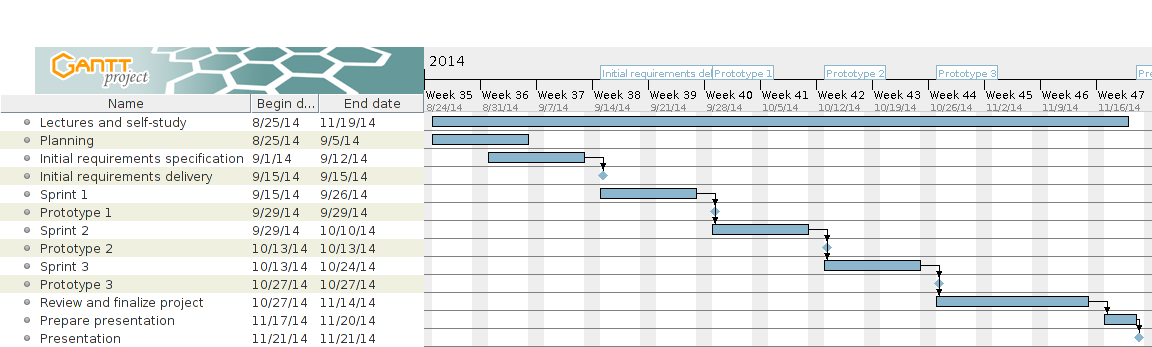
\includegraphics[width=\textwidth]{gantt.png}
\caption{Gantt Diagram}
\end{figure}

\paragraph{Sprint Overview} \ \\
As we have already said and as it can be seen from the gantt diagram, we plan on having three sprints. Each sprint will consist of a sprint backlog, which will split the goals of that sprint into tasks that we need to do in that sprint. This will serve to provide estimated working hours for the group. All the information that is relevant to each sprint will be provided as a separate chapter in this document. 

\paragraph{Sprint Meetings} \ \\
When we start with the sprints, the sprint meetings will be held on:

\begin{table}[H]
\begin{tabular}{ll}
\hline
Tuesday	&	16:00 - 18:00 \\
Friday		&	8:00 - 10:00 \\
\hline
\end{tabular}
\end{table}
When the sprints start these meetings will be held instead of our normal internal meetings to discuss how the sprint is progressing, report any issues and discuss what we will be working on next.

\paragraph{Planned Meetings} \ \\
Internal meetings are planned in accordance to the schedule below:

\begin{table}[H]
\begin{tabular}{ll}
\hline
Monday 	&	12:00 - 18:00 \\
Tuesday 	&	16:00 - 18:00 \\
Wednesday 	&	08:00 - 13:00, 14:00 - 16:00 \\
Friday 	&	08:00 - 16:00 \\
\hline
\end{tabular}
\end{table}
Adviser meetings are planned every week on Wednesday at 13:00. These will last one hour after which our regular internal meeting will continue.

Meetings with the customer are planned on a weekly basis, however, it is not possible for us to set a specific time for the meeting. These meetings will also last for one hour and may or may not be allocated in the time slot for internal meetings.

\subsubsection{Measurement of Project Effort}
The measure of the success or failure of the project comes directly from the success or failure of the project goals. We can consider this project a success if we are able to record data with the sensors and visualize this data by any kind of visualization method. Committing to and meeting our own milestones is something that should indicate if our project is doing well or if we need to put more effort into the project.

\subsubsection{Risks and Risk Mitigation}
\label{risks_and_risk_mitigation}
Below are structured representations of risks that we have identified in this project, alongside their probabilities as well as strategies and actions we can use to mitigate the risks.

\begin{table}[H]
\caption{Risk table legend}
\begin{tabularx}{\textwidth}{|l|X|}
\hline
Number
&Identification of the risk factor
\\ \hline Activity
&The activity affected by the risk.
\\ \hline Risk Factor
&A short description of the risk factor.
\\ \hline Consequence
&The consequence of the event occurring given as either high (H), medium (M) or low (L). A description of the consequence.
\\ \hline Probability
&The probability that the event will occur given as either high (H), medium (M) or low (L).
\\ \hline Strategy and Actions
&Which strategy that is selected taken from the following list: Avoid, Transfer, Reduce, or Accept. Following is a description of the measure.
\\ \hline Deadline
&A date set for taking precautions to deal with the risk.
\\ \hline Responsible
&The person responsible for the risk.
\\ \hline
\end{tabularx}
\end{table}

\begin{table}[H]
\caption{Risk 1}
\begin{tabularx}{\textwidth}{|l|X|}
\hline
Number
&1
\\ \hline Activity
&All
\\ \hline Risk Factor
&Our customer may not be able to deliver sensors on time, or at all.
\\ \hline Consequence
&H: We will only be able to work with made up data, or we will need to work with some other sensors, such as phones, which will severely diminish the quality of the project.
\\ \hline Probability
&M
\\ \hline Strategy and Actions
&Accept. We have no control over getting the sensors or not. In the case we do not get any sensors, we will use android phones, as suggested by our customer. The android phone will then be the sensors and we will have to make an application for the android phone. This will force half of the group to learn how to make app’s for android phones, as none of us know how to do it.
\\ \hline Deadline
&Continuous
\\ \hline Responsible
&Customer, Everyone in the group
\\ \hline 
\end{tabularx}
\end{table}

% Last change: Audun Sutterud, 2014-11-07
\begin{table}[H]
\caption{Risk 2}
\begin{tabularx}{\textwidth}{|l|X|}
\hline
Number
&2
\\ \hline Activity
&All
\\ \hline Risk Factor
&New Technologies. It may become necessary to work with technology that the group has little or no previous experience with.
\\ \hline Consequence
&M: A considerable amount of time needs to be invested into acquiring knowledge of the new technology. This will result in less time being spent on the rest of the project, and will decrease the overall project quality.
\\ \hline Probability
&H
\\ \hline Strategy and Actions
&Accept. Two or three group members will do a preliminary investigation of the new technology. The knowledge gained from this effort shall be documented and made available to the rest of the group.
\\ \hline Deadline
&Continuous
\\ \hline Responsible
&Audun Sutterud
\\ \hline 
\end{tabularx}
\end{table}

\begin{table}[H]
\caption{Risk 3}
\begin{tabularx}{\textwidth}{|l|X|}
\hline
Number
&3
\\ \hline Activity
&All
\\ \hline Risk Factor
&We use external services, like Google Drive and Git which we have no control over.
\\ \hline Consequence
&L: We may experience a loss of data if these services go down.
\\ \hline Probability
&L
\\ \hline Strategy and Actions
&Transfer. To minimize the risk we will make frequent backups of data on a personal machine run by the group member in charge of this risk. These systems are also stored on the cloud, providing an alternative source of backup.
\\ \hline Deadline
&Continuous
\\ \hline Responsible
&Shimin Sun
\\ \hline 
\end{tabularx}
\end{table}

\begin{table}[H]
\caption{Risk 4}
\begin{tabularx}{\textwidth}{|l|X|}
\hline
Number
&4
\\ \hline Activity
&All
\\ \hline Risk Factor
&Group members may have to stop working if they are sick.
\\ \hline Consequence
&M: The specific team member will not be available for work and this may shift the workload to other members.
\\ \hline Probability
&L
\\ \hline Strategy and Actions
&Reduce. If a group member is sick, they need to call or send a message as soon as possible, within a day. If the team member is capable of working then they will continue working. If not, then we will distribute their work among the team members that are capable of working, as evenly as possible.
\\ \hline Deadline
&Continuous
\\ \hline Responsible
&Everyone in the group.
\\ \hline 
\end{tabularx}
\end{table}


\begin{table}[H]
\caption{Risk 5}
\begin{tabularx}{\textwidth}{|l|X|}
\hline
Number
&5
\\ \hline Activity
&All
\\ \hline Risk Factor
&Absence from meeting because of other schedules.
\\ \hline Consequence
&L: Not enough time is spent on the project and the quality of the project will decrease.
\\ \hline Probability
&L
\\ \hline Strategy and Actions
&Reduce. If one group member is unavailable at a specific time they will need to inform the group as soon as possible, within a day. If their work is not necessary for the group, they will be responsible to deliver their work within a day of the projected work time. If their work is necessary for the group, we will split their task as evenly as possible onto the group members that are present.
\\ \hline Deadline
&Continuous
\\ \hline Responsible
&The group member involved
\\ \hline
\end{tabularx}
\end{table}

\begin{table}[H]
\caption{Risk 6}
\begin{tabularx}{\textwidth}{|l|X|}
\hline
Number
&6
\\ \hline Activity
&All
\\ \hline Risk Factor
&The hardware that we use may break down.
\\ \hline Consequence
&L: We will experience some loss in work and data.
\\ \hline Probability
&L
\\ \hline Strategy and Actions
&Transfer. If our hardware breaks down, we still have the online repository. If our backup computer breaks we will make a backup on another computer in the group.
\\ \hline Deadline
&Continuous
\\ \hline Responsible
&Everyone in the group.
\\ \hline 
\end{tabularx}
\end{table}

\begin{table}[H]
\caption{Risk 7}
\begin{tabularx}{\textwidth}{|l|X|}
\hline
Number
&7
\\ \hline Activity
&All
\\ \hline Risk Factor
&There may be miscommunication between the group and the advisor or the customer about the project.
\\ \hline Consequence
&M: This will affect our performance and we may have to re-make parts of the project.
\\ \hline Probability
&M
\\ \hline Strategy and Actions
&Reduce. If there is miscommunication between the adviser or the customer and the group we will schedule another meeting within three days to try to settle that miscommunication. In the mean time we will prepare alternate answers to the miscommunication and see what the customer or adviser actually wants.
\\ \hline Deadline
&Continuous
\\ \hline Responsible
&Audun Sutterud
\\ \hline 
\end{tabularx}
\end{table}

\begin{table}[H]
\caption{Risk 8}
\begin{tabularx}{\textwidth}{|l|X|}
\hline
Number
&8
\\ \hline Activity
&All
\\ \hline Risk Factor
&Group work may be partitioned wrongly, so that some members have more work than others.
\\ \hline Consequence
&L: The extra work will impact the quality of the project negatively.
\\ \hline Probability
&L
\\ \hline Strategy and Actions
&Reduce. We will hold meetings frequently to check on everyones work load. If there is disparity in the work load we will assign tasks from overworked group members to the underworked group members.
\\ \hline Deadline
&Continuous
\\ \hline Responsible
&Everyone in the group.
\\ \hline 
\end{tabularx}
\end{table}

\subsection{Quality Assurance}
In this section we will specify some quality guidelines to assure high quality of communication and documentation.

\subsubsection{Product Qualities}

\paragraph{Functionality} \ \\
The systems main functionalities are to:
\begin{itemize}
\item
Gather information from the environment.
\item
Send the information from the sensors to the central hub.
\item
Send the information from the central hub to the database.
\item
Visualize this data through image manipulation.
\end{itemize}
\ \newline
These four functionalities are key if our system is to operate.
\newline \ \newline
Gathering information is vital for our system. Without it we can only use mock-up data which on its own is useful as it does allow us to create a system. However, it does not allow us to have any real world implementation of the system. Moreover, it does not allow us to fulfill our goals of modularity, as we can not test the system. We also need to be able to send this data to the central hub which will organize the data by sensors. This data is further sent to the database, which will store the data as JSON objects. Finally, this data is passed into the image visualizer. 

Therefore, we need to be able to create a visualization method, that will visualize the data received through the sensors. These four functional requirements are the only functional requirements our system needs and as such they are top priority when it comes to quality of implementation.

\paragraph{Reliability} \ \\
Our system needs to be able to run continuously for one full day. There is not a large need for reliability of the system and it is not required of us by the customer. That being said the sensors, the central hub, the database and the visualization program should all function continuously through at least a duration of one day. This is so that we may showcase data well through our visualization program.

\paragraph{Usability} \ \\
There is no need for usability in our system. The sensors will function with or without prior knowledge, or even end users present in the room. However, the user can directly influence the visualization by increasing or decreasing the temperature of the environment or turning the light on and off, amongst other things.

\paragraph{Efficiency} \ \\
Our network needs to be capable of transmitting data at least once every five seconds. In addition to that the visualization program should use less than five seconds to react to the change. This is so that we can visualise every change. Other than that, the system need not be highly efficient.

\paragraph{Maintainability} \ \\
As with some of the other requirements, maintainability is not a high priority. Our customer is to decide what they will be using these sensors for in the future, and will provide maintainability for the system when it is necessary. Regarding our project, we do not require any maintainability.

\paragraph{Portability} \ \\
The system needs to be absolutely portable. In other words, it must be able to function in any environment that the sensors can actually work in, from outdoor environments and large auditoriums, to small rooms and corridors. The sensors can be picked up and moved throughout the system at any time and the system should be able to cope and correspond to this. As we will be using Java we will implement the system in an object oriented fashion, which should contribute to the portability of the system.

\subsubsection{Quality Metrics}
\label{subsubsec:quality_metrics}
The quality metrics represent how well our project is implemented, or in other words how well our prototype works in relation to the product qualities.

\paragraph{Functionality} \ \\
Functionality is measure in pass or fail. If a function works fully then it gets a pass. Otherwise it fails. For the program to be fully functional, we need to have four passes: one for gathering information from the environment, one for sending the information from the sensors to the central hub, one for sending and storing the data in the database and one for visualizing the data through image manipulation. If we add any more functionalities they need to be fully implemented and receive a pass in order to be added to the prototype.

\paragraph{Reliability} \ \\
Our prototype needs to work for 24 hours continuously. Any more than this is desirable, but not necessary.

\paragraph{Usability} \ \\
If our UI can be learned within a minute of operating the system, then we will have satisfied the usability metric.

\paragraph{Efficiency} \ \\
If our system is able to collect data every five seconds, store it and visualize it then we will have satisfied the efficiency metric.

\paragraph{Maintainability} \ \\
The prototype does not need to be maintained. We have no metrics related to maintainability.

\paragraph{Portability} \ \\
If our system can handle the introduction or removal of a sensor then we will have satisfied the portability metric.


\subsubsection{Internal Resources}
The following section describes the quality metrics of our code as well as the internal documentation.

\paragraph{Internal Documentation} \ \\
The internal organization of documentation is done through online shared repositories. The repositories we use are Google Drive and GitHub. Programming and documentation related to programming is either shared on GitHub, another online repository, or on Google Drive. With this the group can ensure high quality of documentation and fair division of workload.

\paragraph{Coding Standards} \ \\
In order to reduce the conflicts related to code merge we are going to use coding standards. Coding standards refer to how our code is formatted in the code editor. Standardized code makes it easy to read for others not familiar with the project, and they do not have to go through the nuances of different programmers code formatting.
\newline \ \newline
The ones that we agreed on can be find on this page: \newline
\url{http://google-styleguide.googlecode.com/svn/trunk/javaguide.html}
\newline \ \newline
The files that will be used in the IDEs to format the code can be found here: \newline
\url{https://code.google.com/p/google-styleguide/source/browse/trunk}
\newline \ \newline
Every class should be accompanied by JavaDoc and if necessary should also contain other comments that should make the code more understandable. 

Since we are going to use Git as the code repository we are going to follow the guidelines listed below:
\begin{itemize}
\item
Every commit should be accompanied by a comment that summaries the changes made. 
\item
The summary should be no more than 120 characters and it should describe both the changes that have been made, and why they might be necessary.
\item
Everyone should create a branch for each issue that they are working on and push the branch on the main server. After someone else from the team reviewed the commit the branch can be merged on the master branch.
\item
Before merging with the master branch the developer should make sure that the project will not crash because of the newly introduced changes.
\end{itemize}

\subsubsection{Customer Meetings}
\paragraph{Meeting Time} \ \\
To ensure high quality of communication with the customer, customer meetings will be held on a weekly basis. The meeting with the customer needs to be announced at least 48 hours before the meeting time.

\paragraph{Agenda} \ \\
At least 48 hours before the next customer meeting we will write an agenda for the next meeting so that the customer is informed and is able to provide high quality feedback on our work. The template for the agenda can be located in \appendixfullref{customer_meeting_agenda}.

\paragraph{Minutes of the Meeting} \ \\
The minutes of the customer meeting is to be sent to the customer within 24 hours after the meeting. The minutes will include the customer meeting and will be pending approval from the customer before we can clear the problems from the agenda. The template for the minutes of the meeting can be located in {\color{red} ref:}appendix B 3.

\subsubsection{Advisor Meetings}
\paragraph{Meeting Time} \ \\
To ensure high quality of our work we will meet with the advisor on a weekly basis. This meeting is set at the start of the project and will be held on Wednesdays at 13:00, unless the advisor is unable to meet.

\paragraph{Agenda} \ \\
All of the documents that are necessary to be sent to the advisor should be sent at least 24 hours before the meeting with the advisor. The template for the agenda of the meeting is included in {\color{red} ref:}appendix B 1.

\paragraph{Minutes of  the Advisor Meeting} \ \\
The minutes of the advisor meeting will be sent to the advisor within 24 hours of the meeting held. We will typically not wait for an approval of the minutes by the advisor to continue our work.

\end{document}
